
\documentclass[12pt,a4paper,oneside]{article}
\usepackage[margin=1.2in]{geometry}
\usepackage{appendix}
\usepackage[dvips]{graphicx}
\usepackage{epsfig}
\usepackage{amsmath}
\usepackage{amssymb}
\usepackage{psfrag}
\usepackage[square, comma,sort,numbers]{natbib}
\usepackage{fancyhdr}
\usepackage[nottoc]{tocbibind}
\usepackage{color}
\usepackage{fixltx2e}
\usepackage{pdfpages}
\usepackage{pdflscape}
\usepackage{booktabs}
\usepackage{graphicx}
\usepackage{float}
\usepackage{afterpage}
\usepackage{subcaption}
\usepackage{lscape}
\usepackage{rotating}
\usepackage{enumitem}
\usepackage{array,tabularx}
\usepackage{fancyref}
\usepackage[dvipsnames]{xcolor}
\usepackage[colorlinks=true,allcolors=blue]{hyperref}%


\newcommand{\quotes}[1]{``#1''}

\newenvironment{conditions*}
  {\par\vspace{\abovedisplayskip}\noindent
   \tabularx{\columnwidth}{>{$}l<{$} @{\ : } >{\raggedright\arraybackslash}X}}
  {\endtabularx\par\vspace{\belowdisplayskip}}



\pagestyle{fancy}
\title{\Huge Allen Telescope Array\\
\vspace{0.5cm}
Smart Network ADC Processor\\1U Enclosure\\
\vspace{0.5cm}
\normalsize \emph{}
\vspace{3.5cm}
\begin{center}

\includegraphics[height=4cm]{titlepage/SETI_institute_logo.jpg}
\end{center}
}
\author{ 
\vspace{1cm}
\Large
\textbf{ Alexander Pollak} \\
SETI Institute \\ 
189 Bernardo Ave, Suite 200 \\
Mountain View, CA 94043 \\ 
Alexander.Pollak.87@gmail.com\\
}
\date{\today}



\begin{document}
\clearpage\maketitle
\thispagestyle{empty}

%\newpage
%\thispagestyle{empty}
%\section*{Abstract}
%\noindent 
%



%
%\vspace{3cm}
%\begin{flushright}
%Alexander Pollak \\ \emph{September, 2015}
%\end{flushright}

%\newpage
%\thispagestyle{empty}
%\tableofcontents
\newpage

%----------------------------------------------------------------------------------------
%	SECTION 1
%----------------------------------------------------------------------------------------
%\pagestyle{plain}
\section{General}
\label{sec:1}
% ----------------------------------------------------------------

This document describes the design, component list, and assembly for a 1U SNAP Ver 2.1.1 MAR 2016 enclosure. The design is based on standard components and only requires two modified parts, which can be ordered via Front Panel Express using the included design files. In addition to housing the SNAP board, this design also includes SMA connections to support the ADC 5G V2.0 or any other compatible extension cards. Note, that this enclosure is not EMI-RFI shielded!



%----------------------------------------------------------------------------------------
\section{CAD Design and Drawings}
\label{sec:2}
% ----------------------------------------------------------------
This section includes a description of the CAD design. The enclosure has been designed to support all signal, communication, and power connections from the front. As a result of this, there was not enough space to include cooling fans into the front panel as well. In order to still ensure adequate cooling of the SNAP board and the 5G ADC card, directional fans have been installed which create an airflow from the right-hand side to the left-hand side. This configuration allows the 1U cases to be mounted without any space in between units while still providing sufficient cooling.

An image of the CAD model is shown in Figure \ref{fig:CAD-model}. One can see the internal arrangement of the SNAP board, power supply, directional fans, and the Raspberry Pi 2 Model B. The two custom parts are the front panel and the base plate, both colored in blue. The lid of the enclosure, not shown in this Figure, is perforated to further increase cooling. The drawings for the front panel and base plate are attached at the end of this document.


%
\begin{figure}[H]
\centering{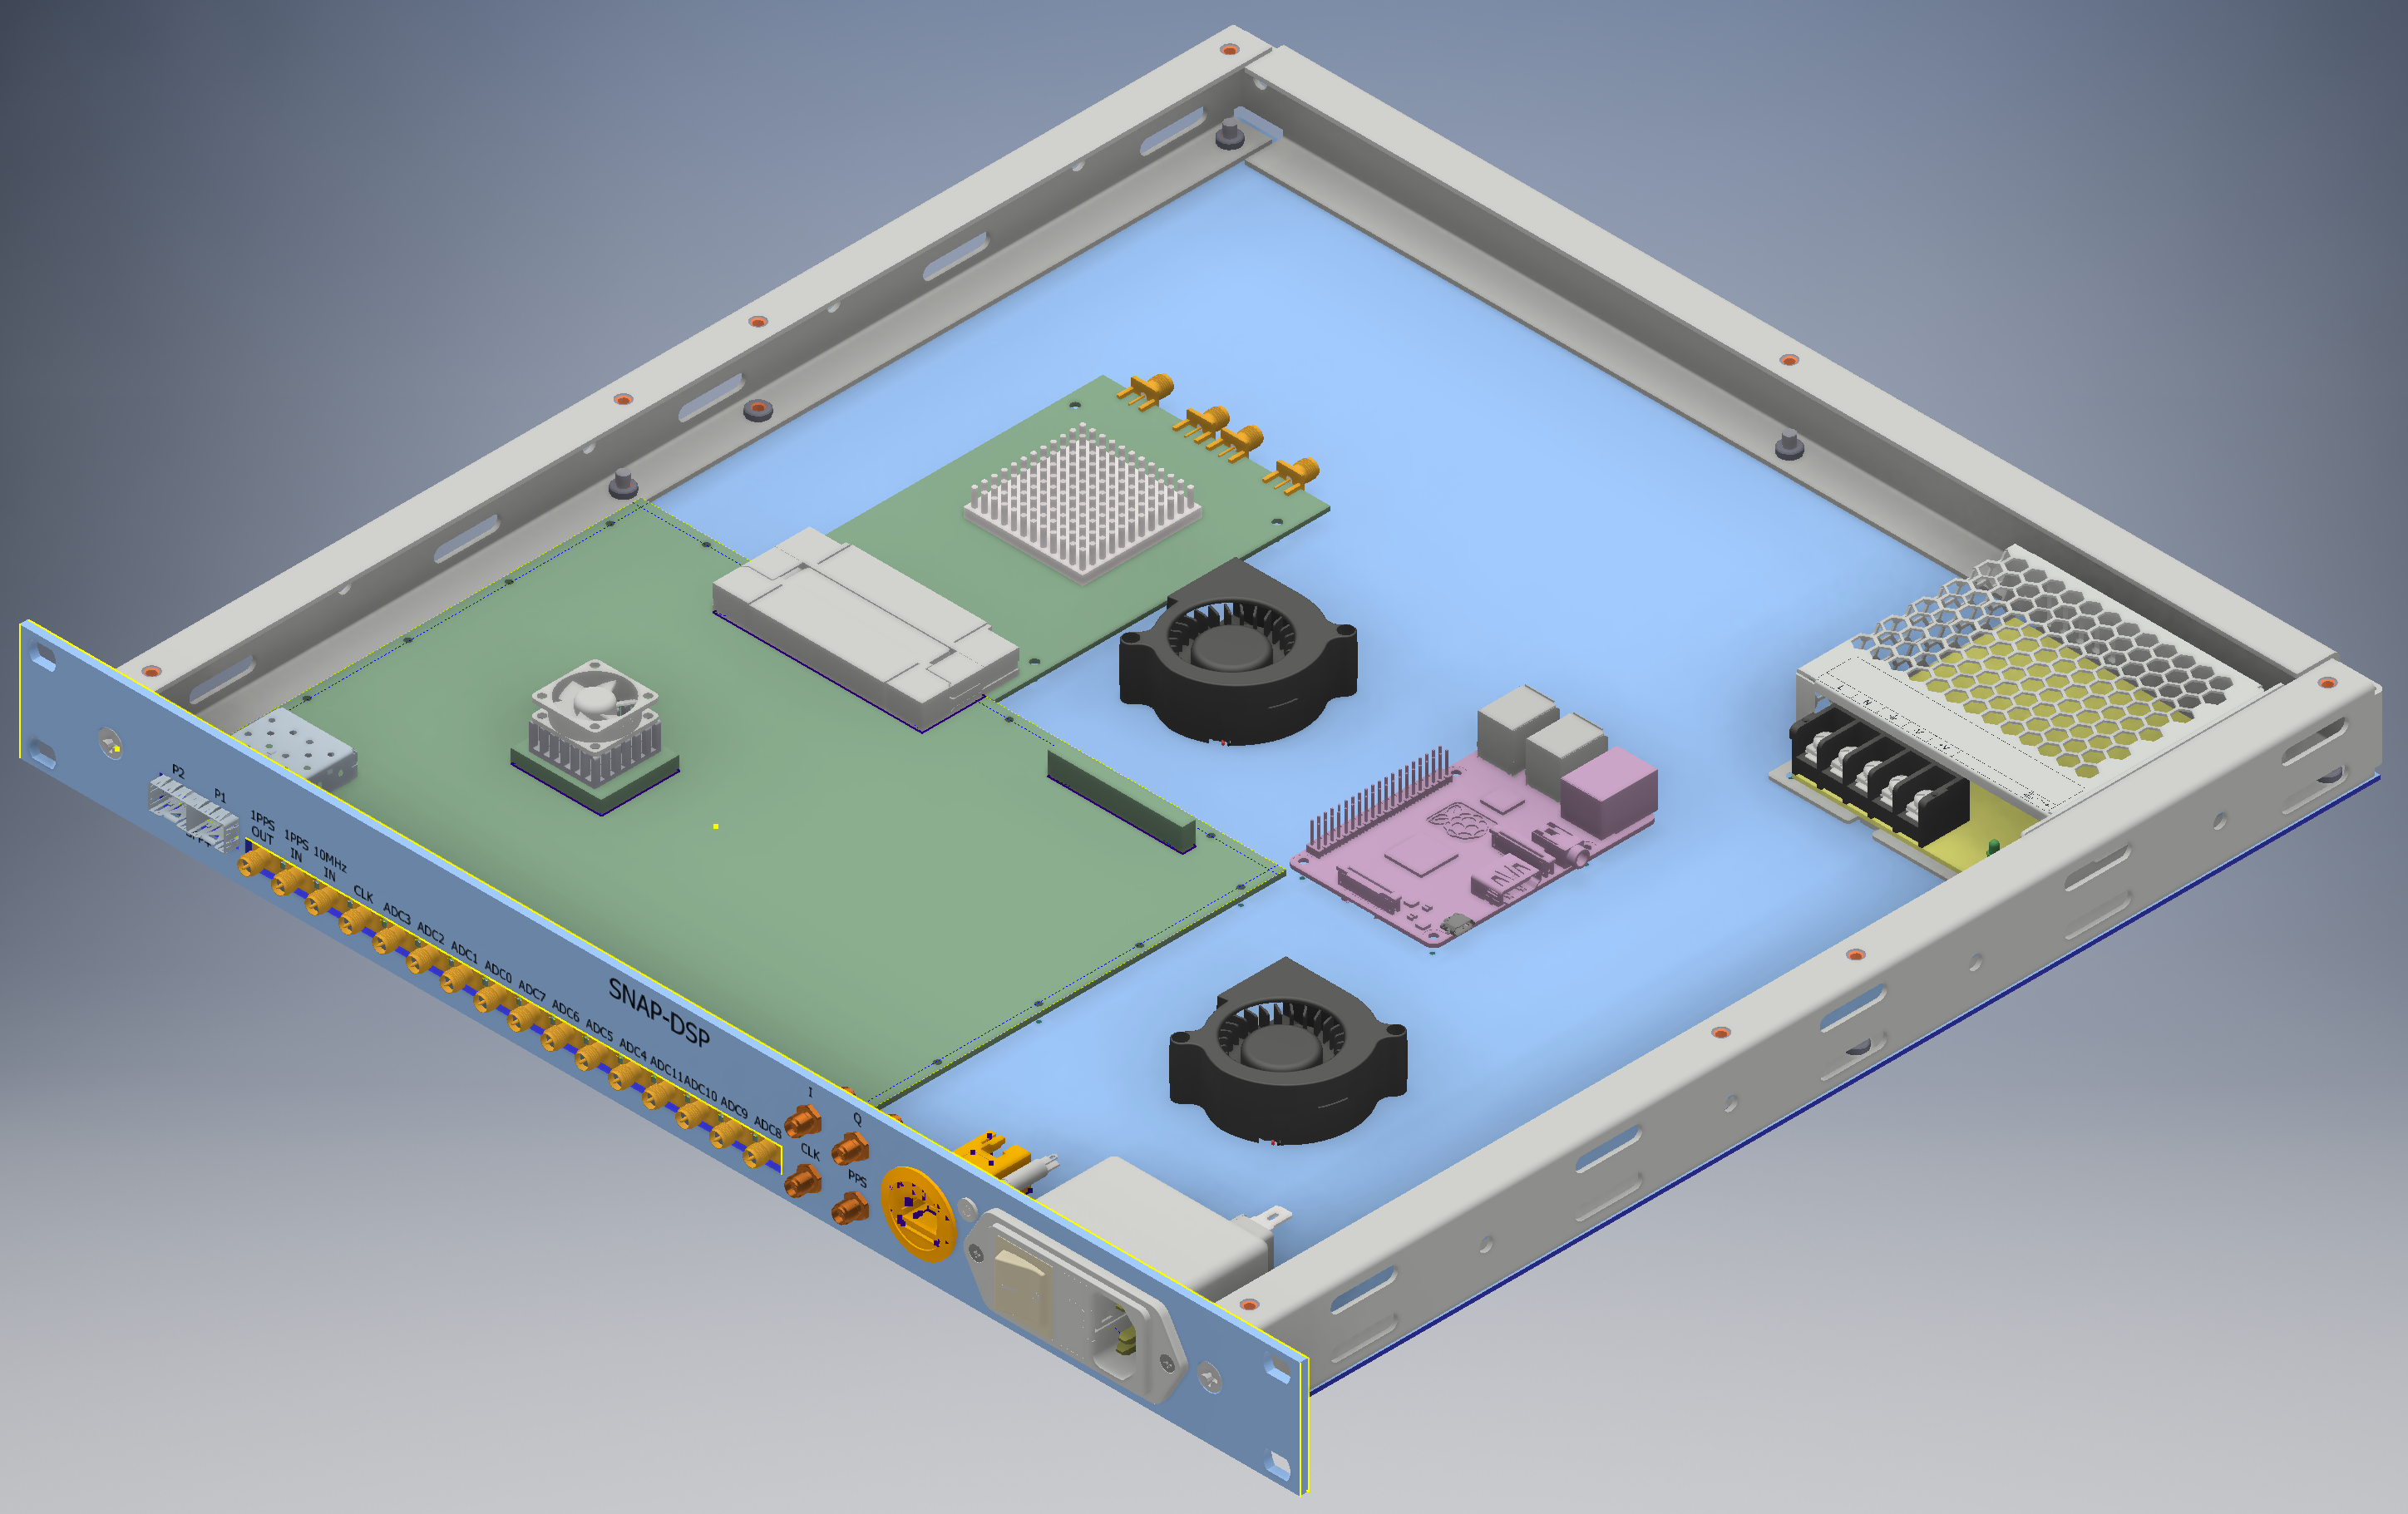
\includegraphics[width=1\linewidth]{figures/VD4001-00-0117.png}}
\caption{Schematic diagram of the measurement setup.}
\label{fig:CAD-model}
\end{figure}
%

\newpage

%----------------------------------------------------------------------------------------
\section{Component List}
\label{sec:3}
% ----------------------------------------------------------------
This section includes a list of the required components including their manufacturer and US distributer. The front panel and base plate can be ordered via {\color{blue} https://www.frontpanelexpress.com} by uploading the design files {\color{blue} VC4039-00-0001.fpd} and {\color{blue} VC4084-00-0018.fpd}. Not included are the SNAP board, 5G ADC card, and power supply cable from the PSU to the SNAP board. The total component cost for the enclosure is approximately 680\,USD.




\begin{table}[H]
\caption{Component List 1U SNAP Enclosure}
\resizebox{\textwidth}{!}{%
\begin{tabular}{@{}lllllll@{}}
\toprule
 Qty & Unit & Description                                              & Manufacturer             & PN Manufacturer & Distributor       & PN Distributer \\ \midrule
          &      &                                                          &                          &                             &                   &                             \\
1        & Each & LRS-75-12 -  POWER SUPPLY, AC-DC, 12V, 6A                	& Mean Well                		& LRS-75-12                   	& Newark            	& 44AC5561 \\
1        & Each & CHA-01-17, D-4001 1.75" Utility Chassis                  		& General Devices          		& CHA-01-17                   	& Quail Electronics 	& CHA-01-17 \\
1        & Each & Power Entry Module, Compact, IEC Inlet, 6A, 250VAC       	& SCHAFFNER                		& FN282-6-06                  	& Newark            	& 24M2150    \\
1        & Pack & Machine Screw, M3, 6 mm                                  			& TR FASTENINGS            	& M3 6 KRSTMC Z100	& Newark            	& 53M8781    \\
1        & Pack & SCREW, PAN HEAD PZ, M3, 4MM, 50PK                        	& DURATOOL                 		& DT000376                    	& Newark            	& 48AC6542  \\
1        & Pack & Machine Screw, M3, 25 mm                                 			& TRIPP-LITE         			& N001-S02-BL       		& Newark            	& 81Y0762  \\
1        & Each & Modular Connector, RJ45 Plug                             			& SCHNEIDER ELECTRIC       & XB5PRJ45                    	& Newark            	& 49AC2992  \\
1        & Each & Ethernet Cable, Cat5e, 600 mm, 2 ft                            		& SCHNEIDER ELECTRIC       & XB5PRJ45                    	& Newark            	& 49AC2992  \\
1        & Each & RPI2-MODB-V1.2                                           			& RASPBERRY-PI             	& RPI2-MODB-V1.2        	& Newark            	& 95Y1948    \\
1        & Each & GPIO Ribbon Cable for Raspberry Pi                       		& SAMTEC                   		& FFSD-20-D-04.00-01-N	& Newark            	& 99P5134    \\
1        & Each & ED Panel Mount Indicator, Green                          			& APEM                     		& Q6F3CXXG12E            	& Newark            	& 05W8310    \\
2        & Each & Fan Blower, GB Series, Compact, 12 V, DC                 		& SUNON                    		& GB1205PKV1-8AY.GN	& Newark            	& 96M8138     \\
18      & Each & SPACER, ROUND, POLYAMIDE, 4MM                           	& WURTH ELEKTRONIK         	& 960040010                  	& Newark            	& 94AC5835    \\
1        & Pack & SCREW, PAN HEAD PZ, M2, 8MM, 50PK                        	& DURATOOL                 		& DT000367                    	& Newark            	& 48AC6533      \\
1        & Pack & Washer, Plain, Brass, M2, Pack of 100                    		& DURATOOL                 		& M2 WASHER        		& Newark            	& 03P2386         \\
4        & Each & SMA Female to Female Adaptor Frequency: DC-6GHz          & Atlantic RF              		& SMA-1064 Rev A         	&                   &                             \\
4        & Each & Coaxial Cable Assemblies Standard Lengths - AFX Series   	& Atlantic RF              		& AFX-CA-141-24            	&                   &                             \\
1        & Each & Frontpanel                                               				& Front Panel Express, LLC 	& VC4039-00-0001.fpd     	&                   &                             \\
1        & Each & Base Plate                                               				& Front Panel Express, LLC 	& VC4084-00-0018.fpd    	&                   &                             \\
2        & Each & Fuse, Cartridge, Slow Blow, 2 A, 250 V                   		& Littlefuse               			& 0239002.HXP              	& Newark            	& 26K8412    \\
5        & Each & 8-32 X 3/8 STEEL ROUNDHEAD                               		& GC ELECTRONICS           	& KF-479                      	& Newark           	& 68R7355   \\
1        & Each & Barrier Terminal Block Connectors, Jumper, 38723 Series  	& MOLEX                    		& 38723-6502                  	& Newark            	& 72K2052    \\
7        & Each & Terminal, Locking, CLS Series, 22AWG to 18AWG, M3.5 	& MULTICOMP                		& CLS-TV-1806                 & Newark            	& 14T2409     \\ \bottomrule            
\end{tabular}}
\end{table}




%----------------------------------------------------------------------------------------
%	Power supply
%----------------------------------------------------------------------------------------
\section{Power Supply}
\label{sec:5}
% ----------------------------------------------------------------

The SNAP FPGA board and the cooling fans are supplied with a Mean Well 75\,W switch-mode PSU.
The unit is mounted directly to the base plate of the enclosure, thereby using the case as a thermal heatsink.
The operating temperature range of the PSU is from $-30^{\circ}$C through $70^{\circ}$C and the technical specifications are shown in Table \ref{tab:psu_spec}.
The power entry module, mounted in the front panel, combines an IEC inlet and a mains filter with a dual-fuse holder. The AC supply fuse current rating for this unit is selected to be 2\,A. 



\begin{table}[H]
\centering
\caption{Power Supply Specification}
\label{tab:psu_spec}
\begin{tabular}{@{}ccccc@{}}
\toprule
\multicolumn{1}{l}{Description} & \multicolumn{1}{l}{Output Voltage} & \multicolumn{1}{l}{Output Current} & \multicolumn{1}{l}{Power W} & \multicolumn{1}{l}{Input Voltage} \\ \midrule
LRS-75-12                         & 12\,VDC                               & 6A                               & 75W                         & $85 \sim 264\,\rm{VAC}$                              \\ \bottomrule
\end{tabular}
\end{table}



%----------------------------------------------------------------------------------------
%	Assembly
%----------------------------------------------------------------------------------------
\section{Assembled Unit}
\label{sec:6}
% ----------------------------------------------------------------
\begin{figure}[H]
\centering
   \begin{subfigure}[b]{1\textwidth}
   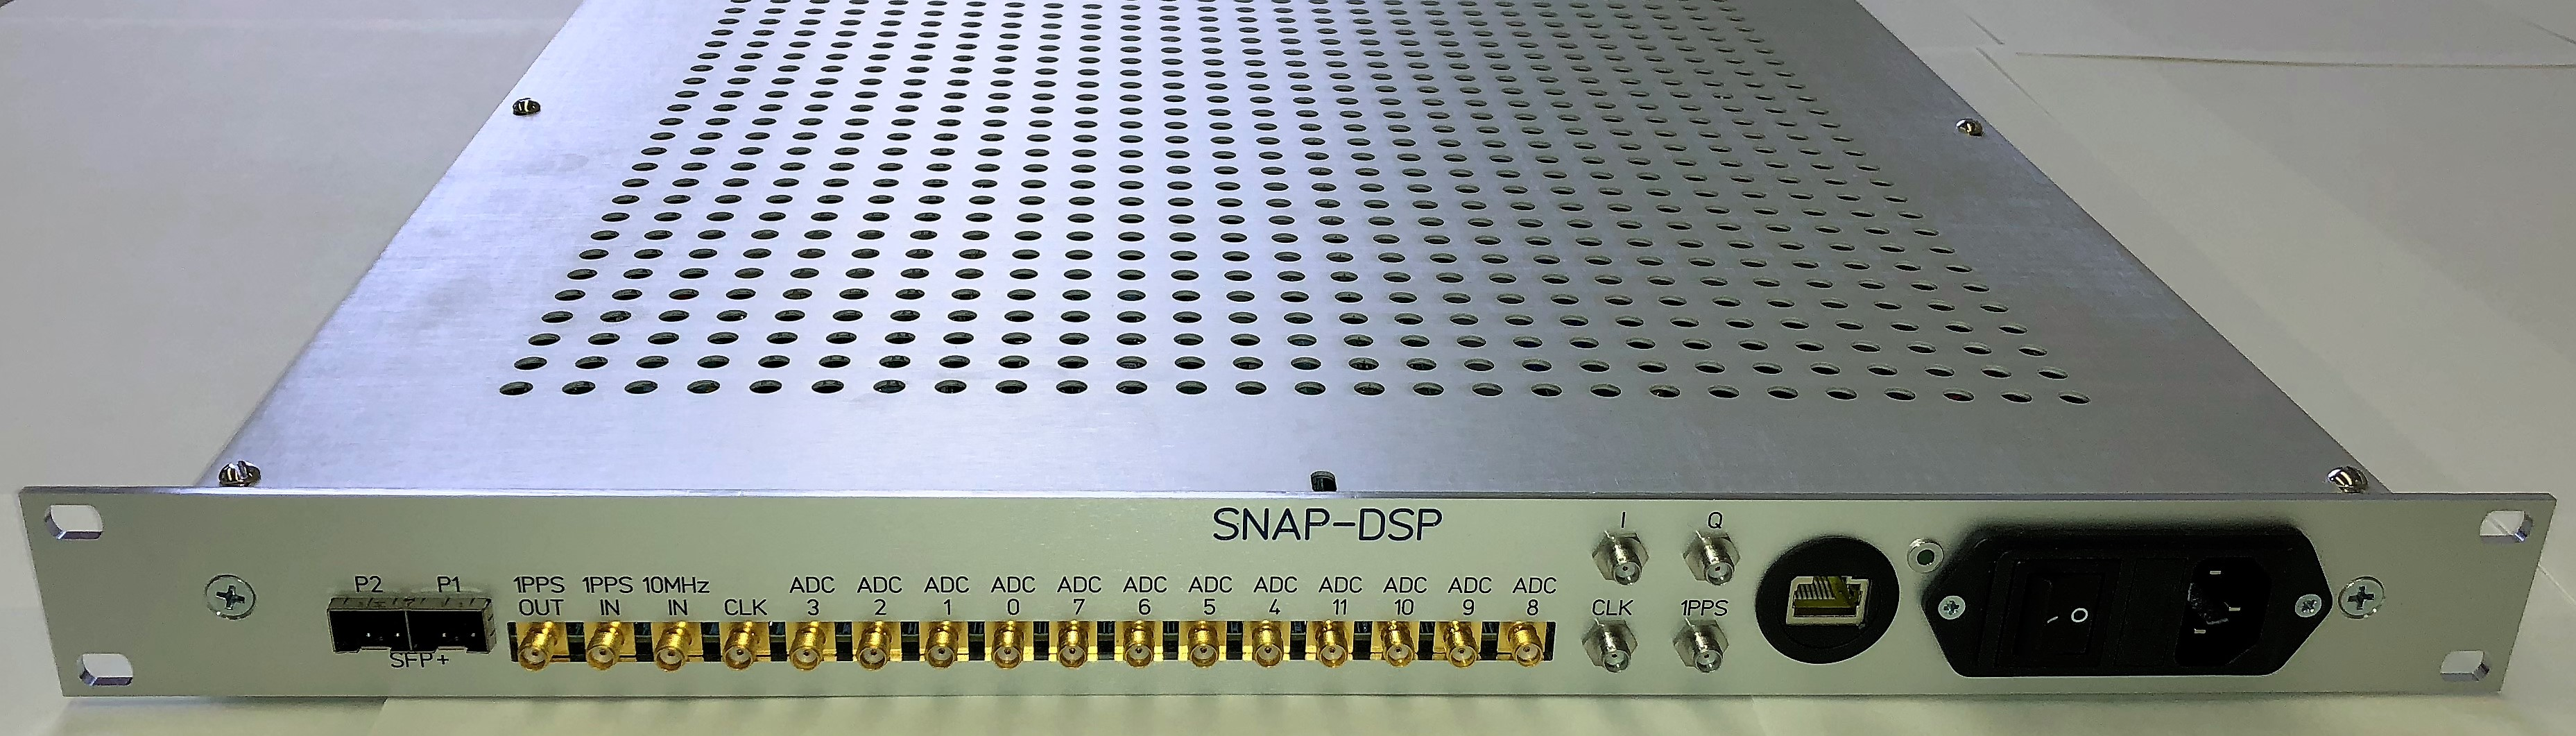
\includegraphics[width=1\linewidth]{figures/front.jpeg}
   \caption{}
   \label{fig:front-view} 
\end{subfigure}
\begin{subfigure}[b]{1\textwidth}
	\vspace{1cm}
   \includegraphics[width=1\linewidth]{figures/iso-closed.jpeg}
   \caption{}
   \label{fig:iso-view}
\end{subfigure}
\caption[Three numerical solutions]{Assembled 1U SNAP Enclosure; (a) Front view (b) Iso view.}
\label{fig:assembled-unit}
\end{figure}

%
\begin{figure}[H]
\centering{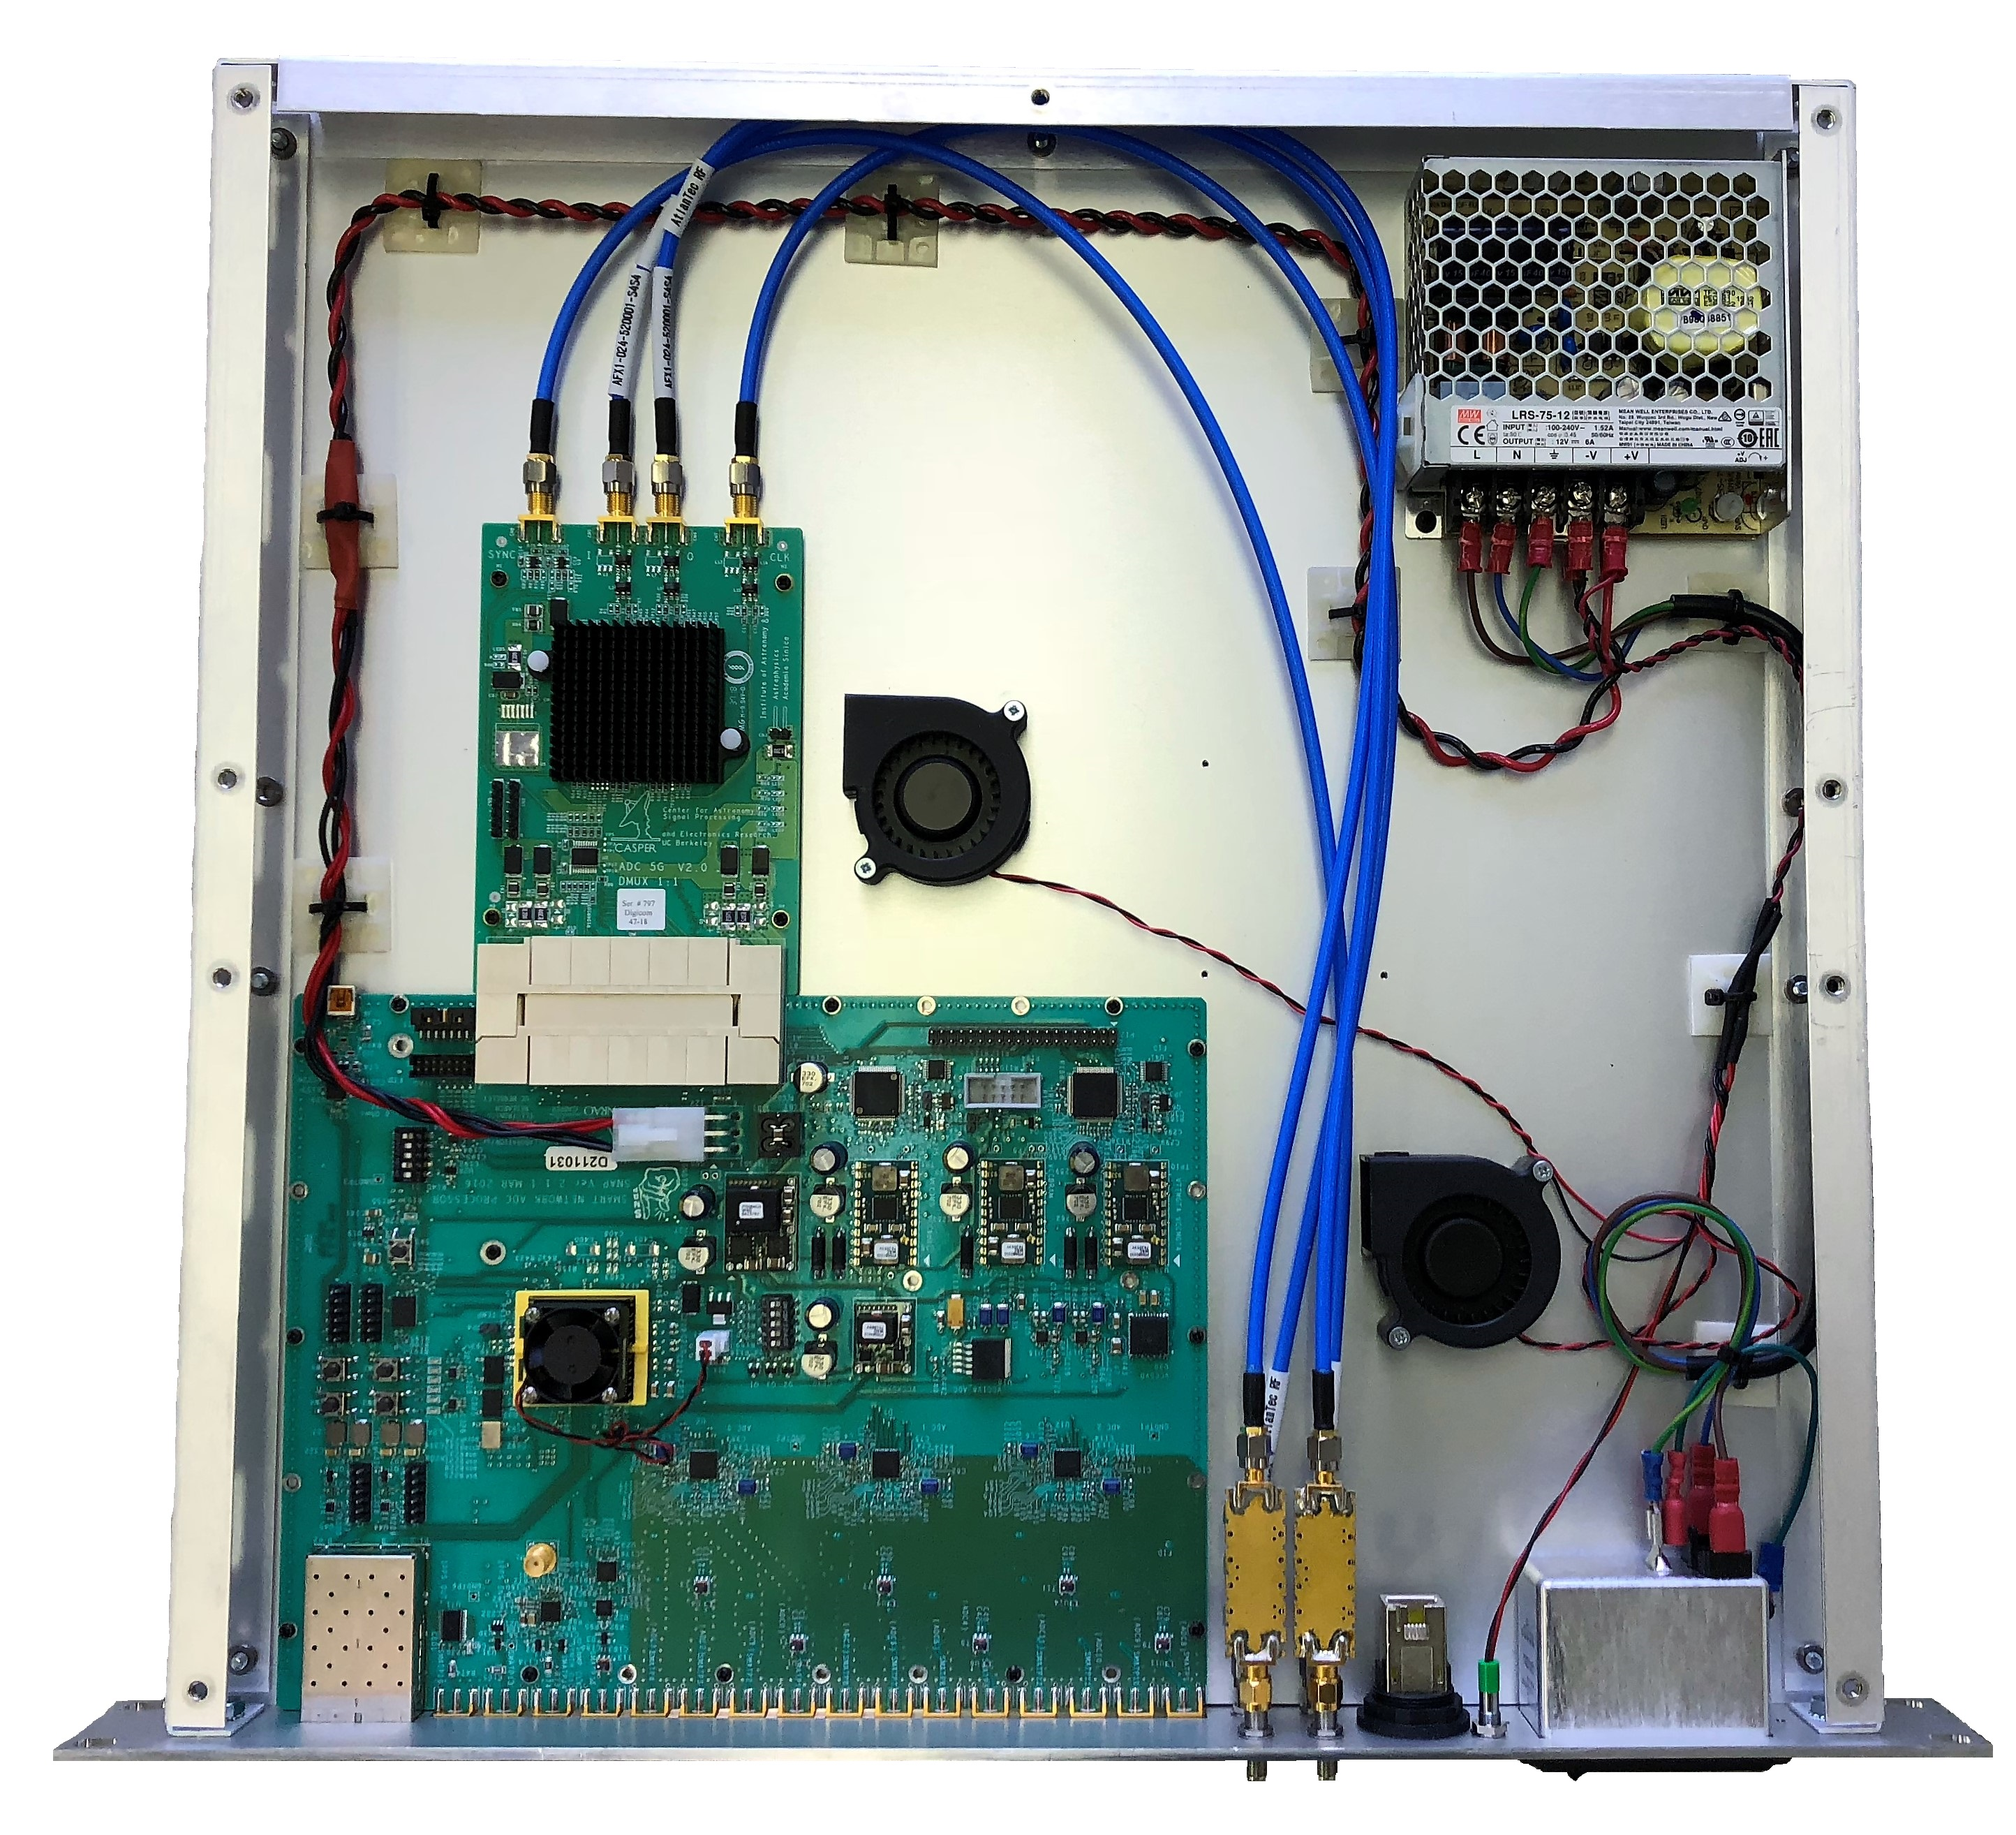
\includegraphics[width=1\linewidth]{figures/top-open.jpeg}}
\caption{Top view of the assembled case with the lid removed. Note that this unit has no Raspberry Pi installed.}
\label{fig:CAD-model}
\end{figure}
%



%----------------------------------------------------------------------------------------
%	APPENDIX
%----------------------------------------------------------------------------------------


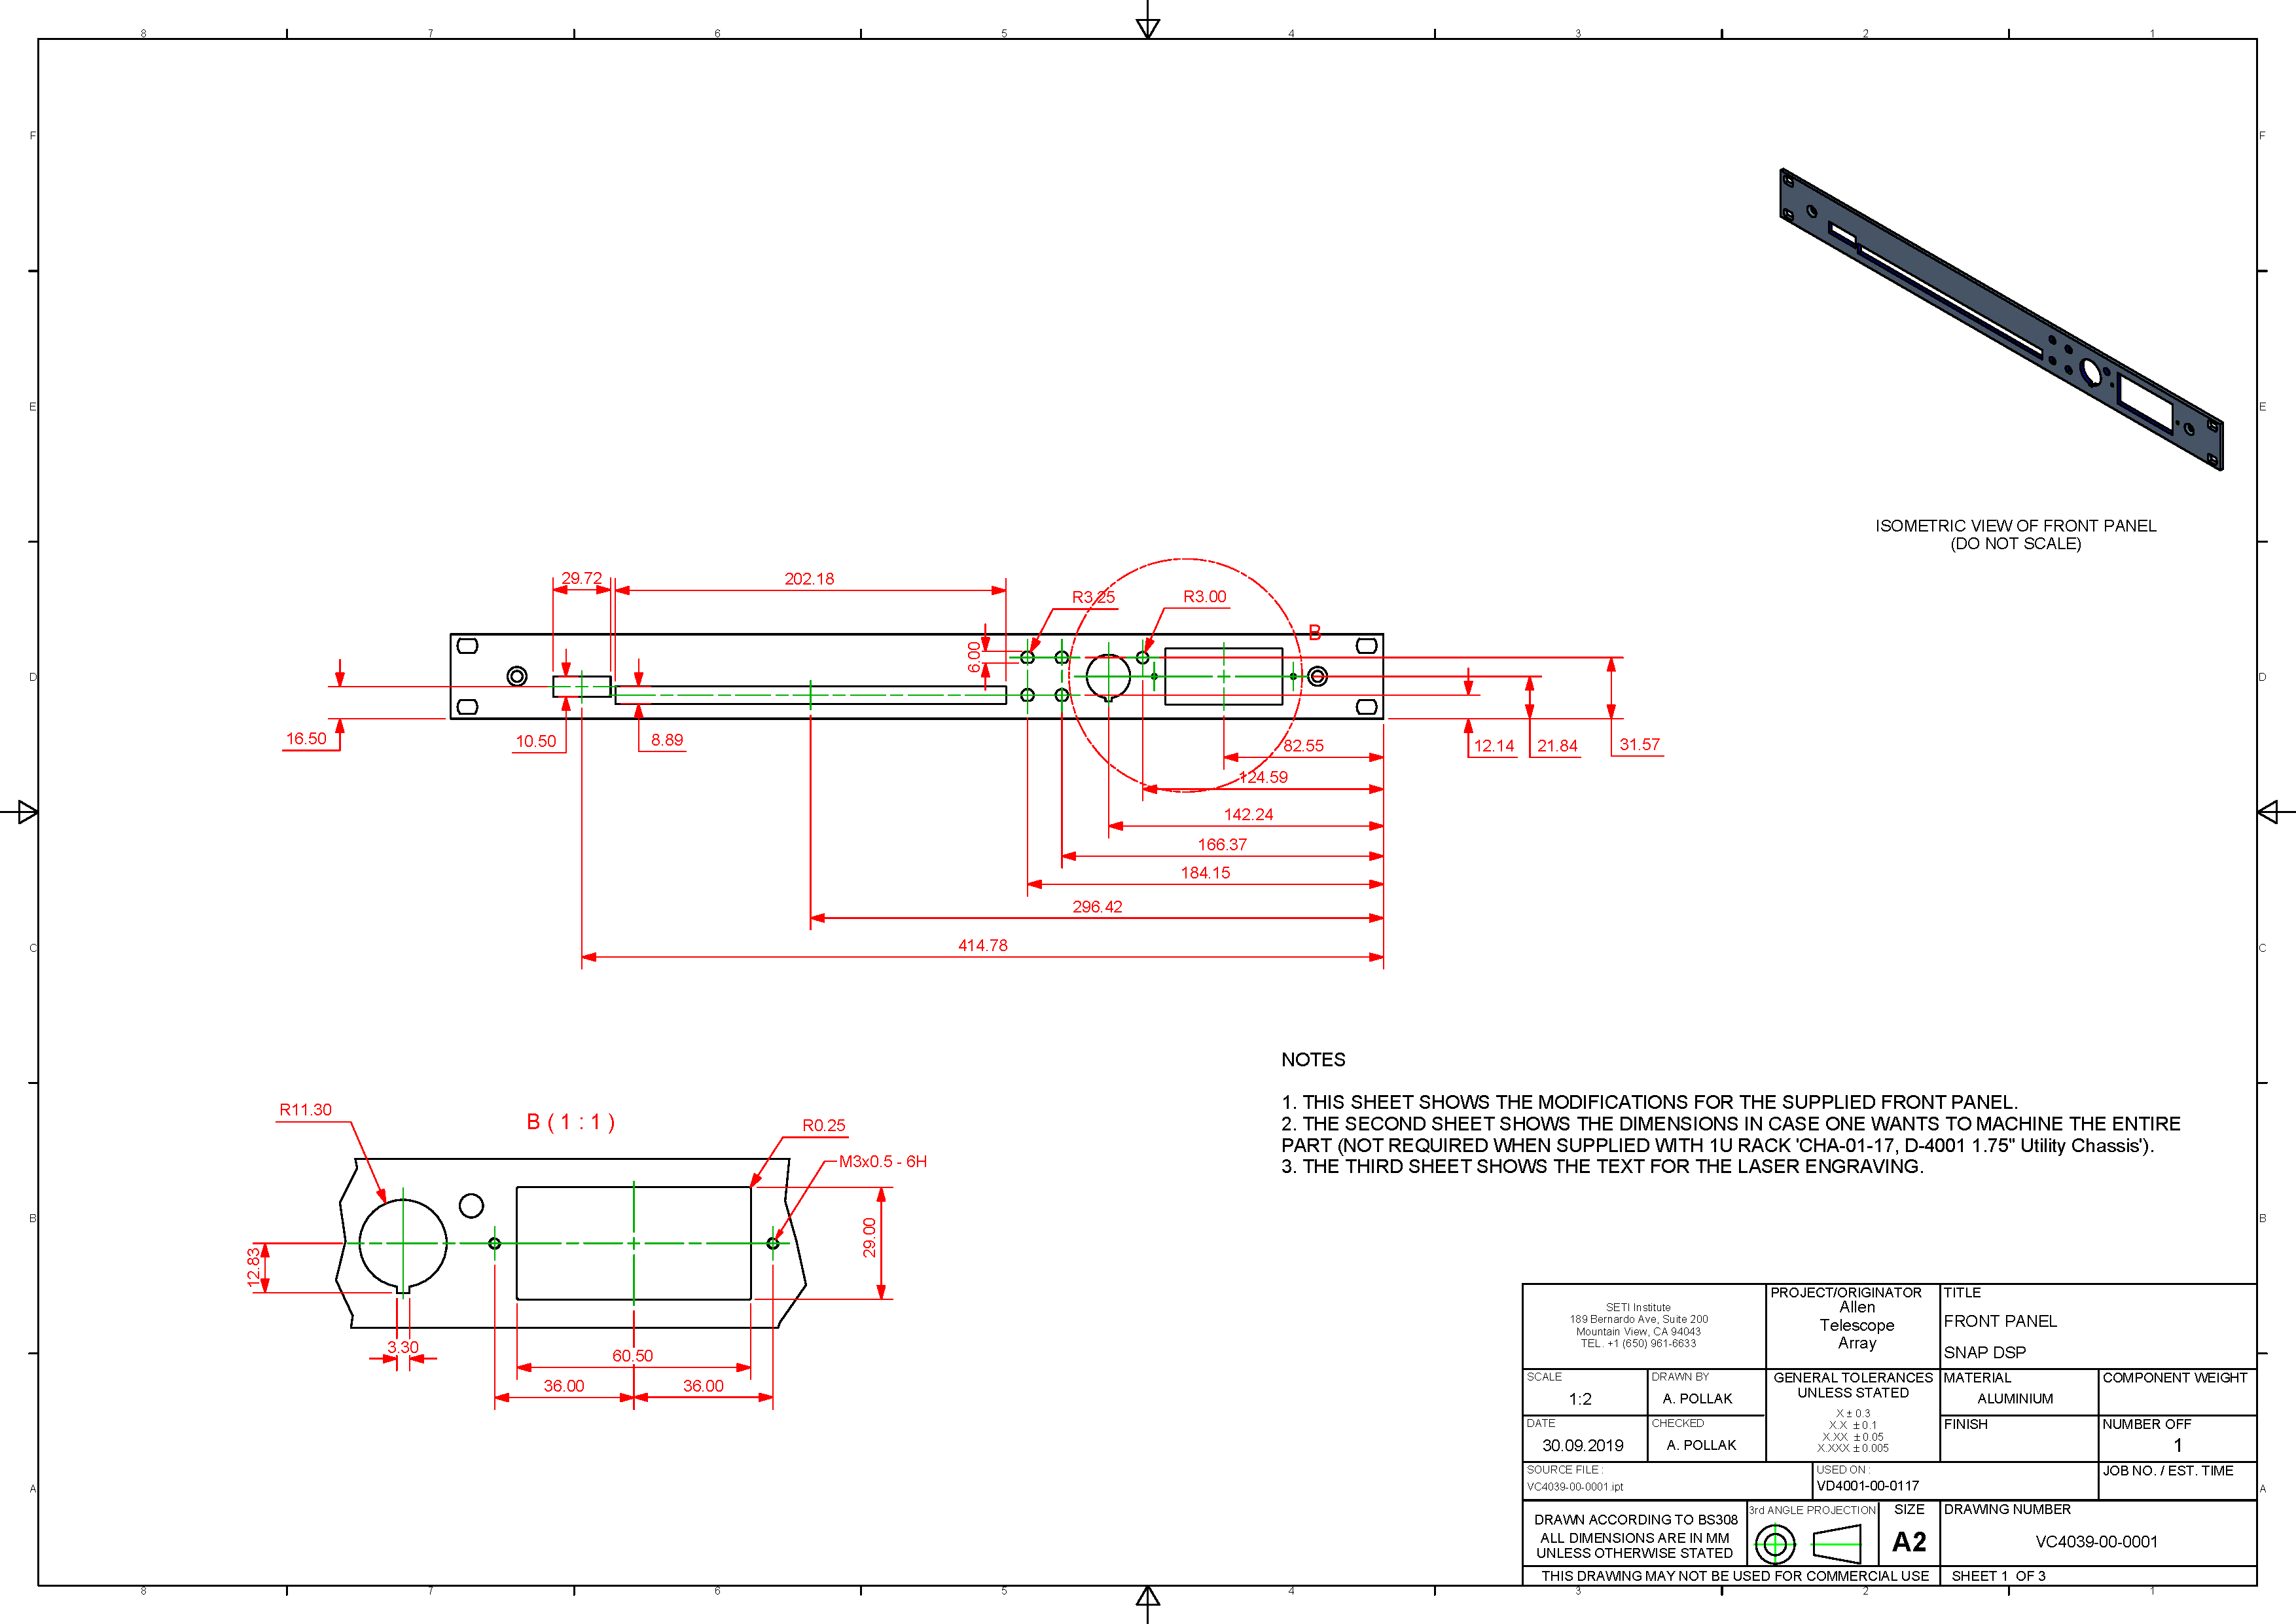
\includepdf[pages={-},fitpaper,rotateoversize]{figures/VC4039-00-0001.pdf}
\label{DRAWING:VC4039-00-0001}
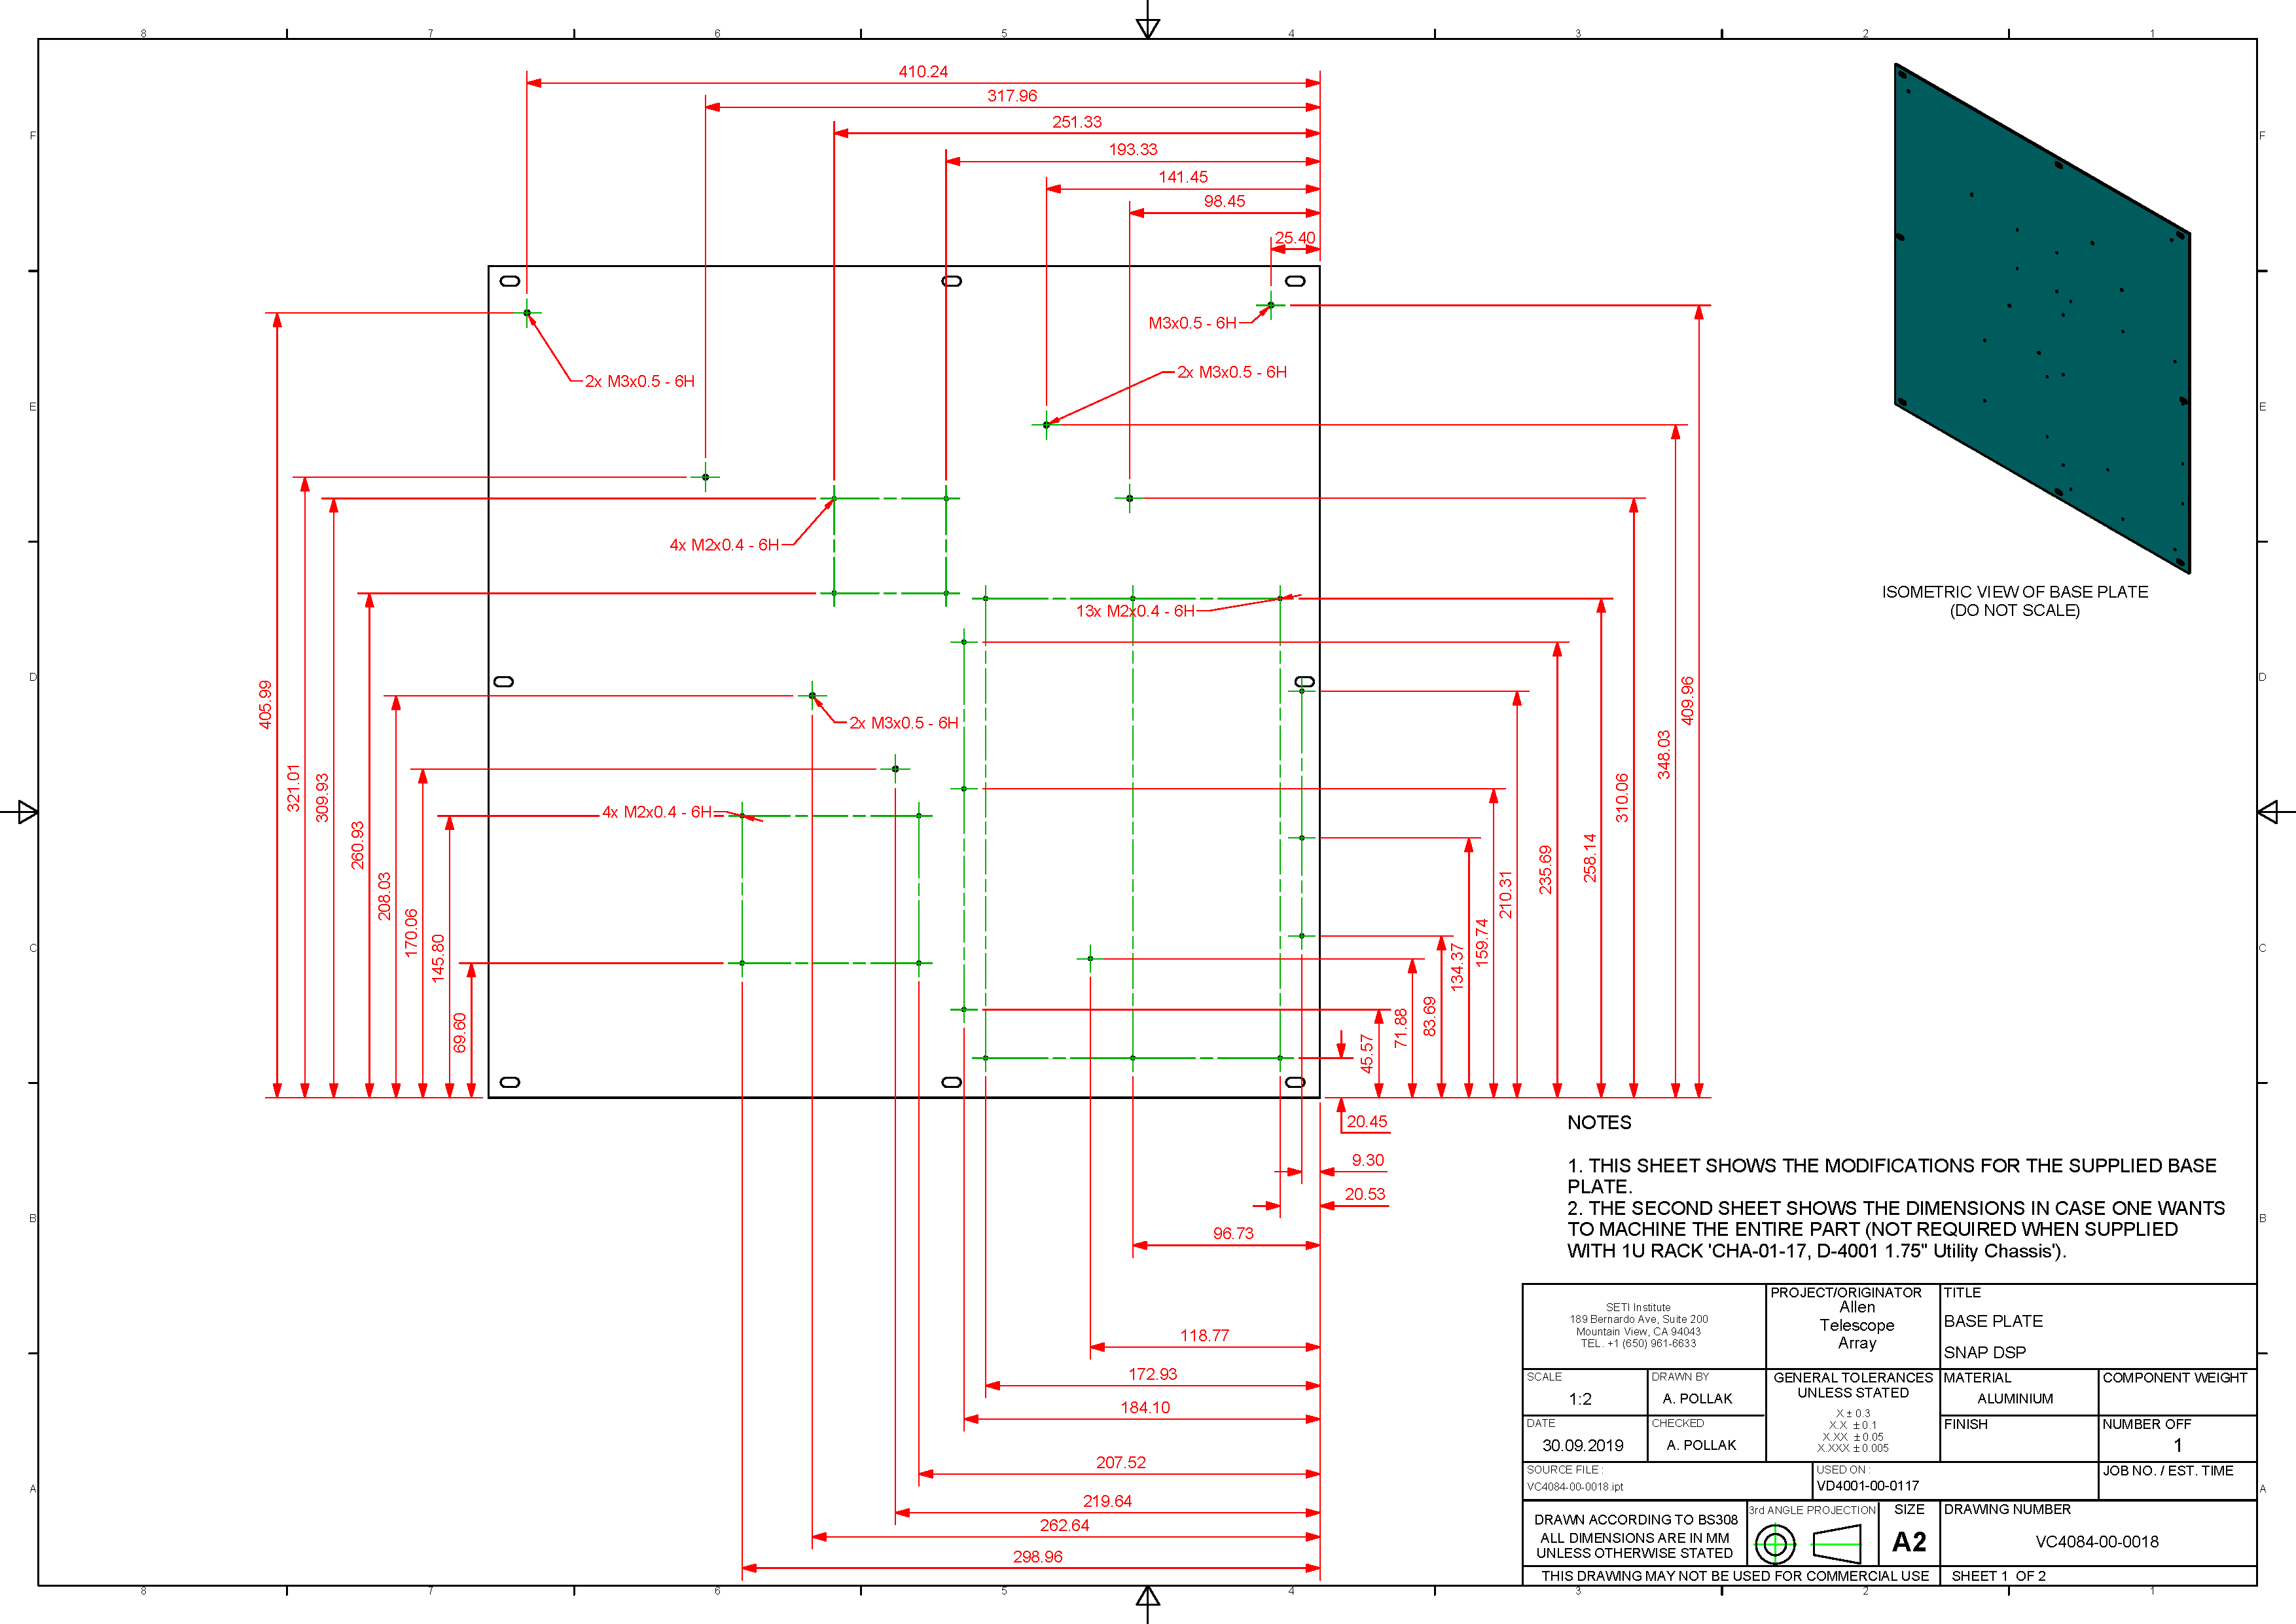
\includepdf[pages={-}, fitpaper,rotateoversize]{figures/VC4084-00-0018.pdf}
\label{DRAWING:VC4084-00-0018}










%----------------------------------------------------------------------------------------
%	BIBLIOGRAPHY
%----------------------------------------------------------------------------------------

%\bibliographystyle{apalike}
%\bibliographystyle{abbrv}

\bibliographystyle{apsrev}
\bibliography{bib_memos}

%----------------------------------------------------------------------------------------



\end{document}
